\documentclass{thesisbeamer}


\usepackage{caption}
\usepackage{comment}
\usepackage{amsmath}
\usepackage{bm}
\usepackage{multicol}
\usepackage{xcolor}
\usepackage{tabularx}
\usepackage{optidef}
\usepackage{mathtools}

\usepackage{comment}
\usepackage{graphicx}
\usepackage{subcaption}
\captionsetup{compatibility=false}

\title[Making Flips with Quadrotors in Constrained Environments]{Making Flips with Quadrotors in Constrained Environments}
\author[Elie Hatem]{Elie Hatem \newline ~ \newline \normalsize{Advisors: Dr. Sébastien Briot \& Dr. Isabelle Fantoni}}
\date{19/01/2021}





\bibliography{../biblio}

% video will work on Linux (with Okular) or OS X, for other OS's or viewers find your own way to do it
%\videoOSX	% for OS X 
\videoOFF

\AtBeginSection[]
{
    \begin{frame}[allowframebreaks]
        \frametitle{Table of Contents}
        \tableofcontents[currentsection]
    \end{frame}
}


\begin{document}

\MakeTitleNoFoot




    \begin{frame}[allowframebreaks]
        \frametitle{Table of Contents}
        \tableofcontents
    \end{frame}


\section{Introduction}

\begin{frame}[t]{Quadrotor Platform} \vspace{4pt}


\begin{figure}[t]
     \centering
     \begin{subfigure}[b]{0.45\textwidth}
         \centering
         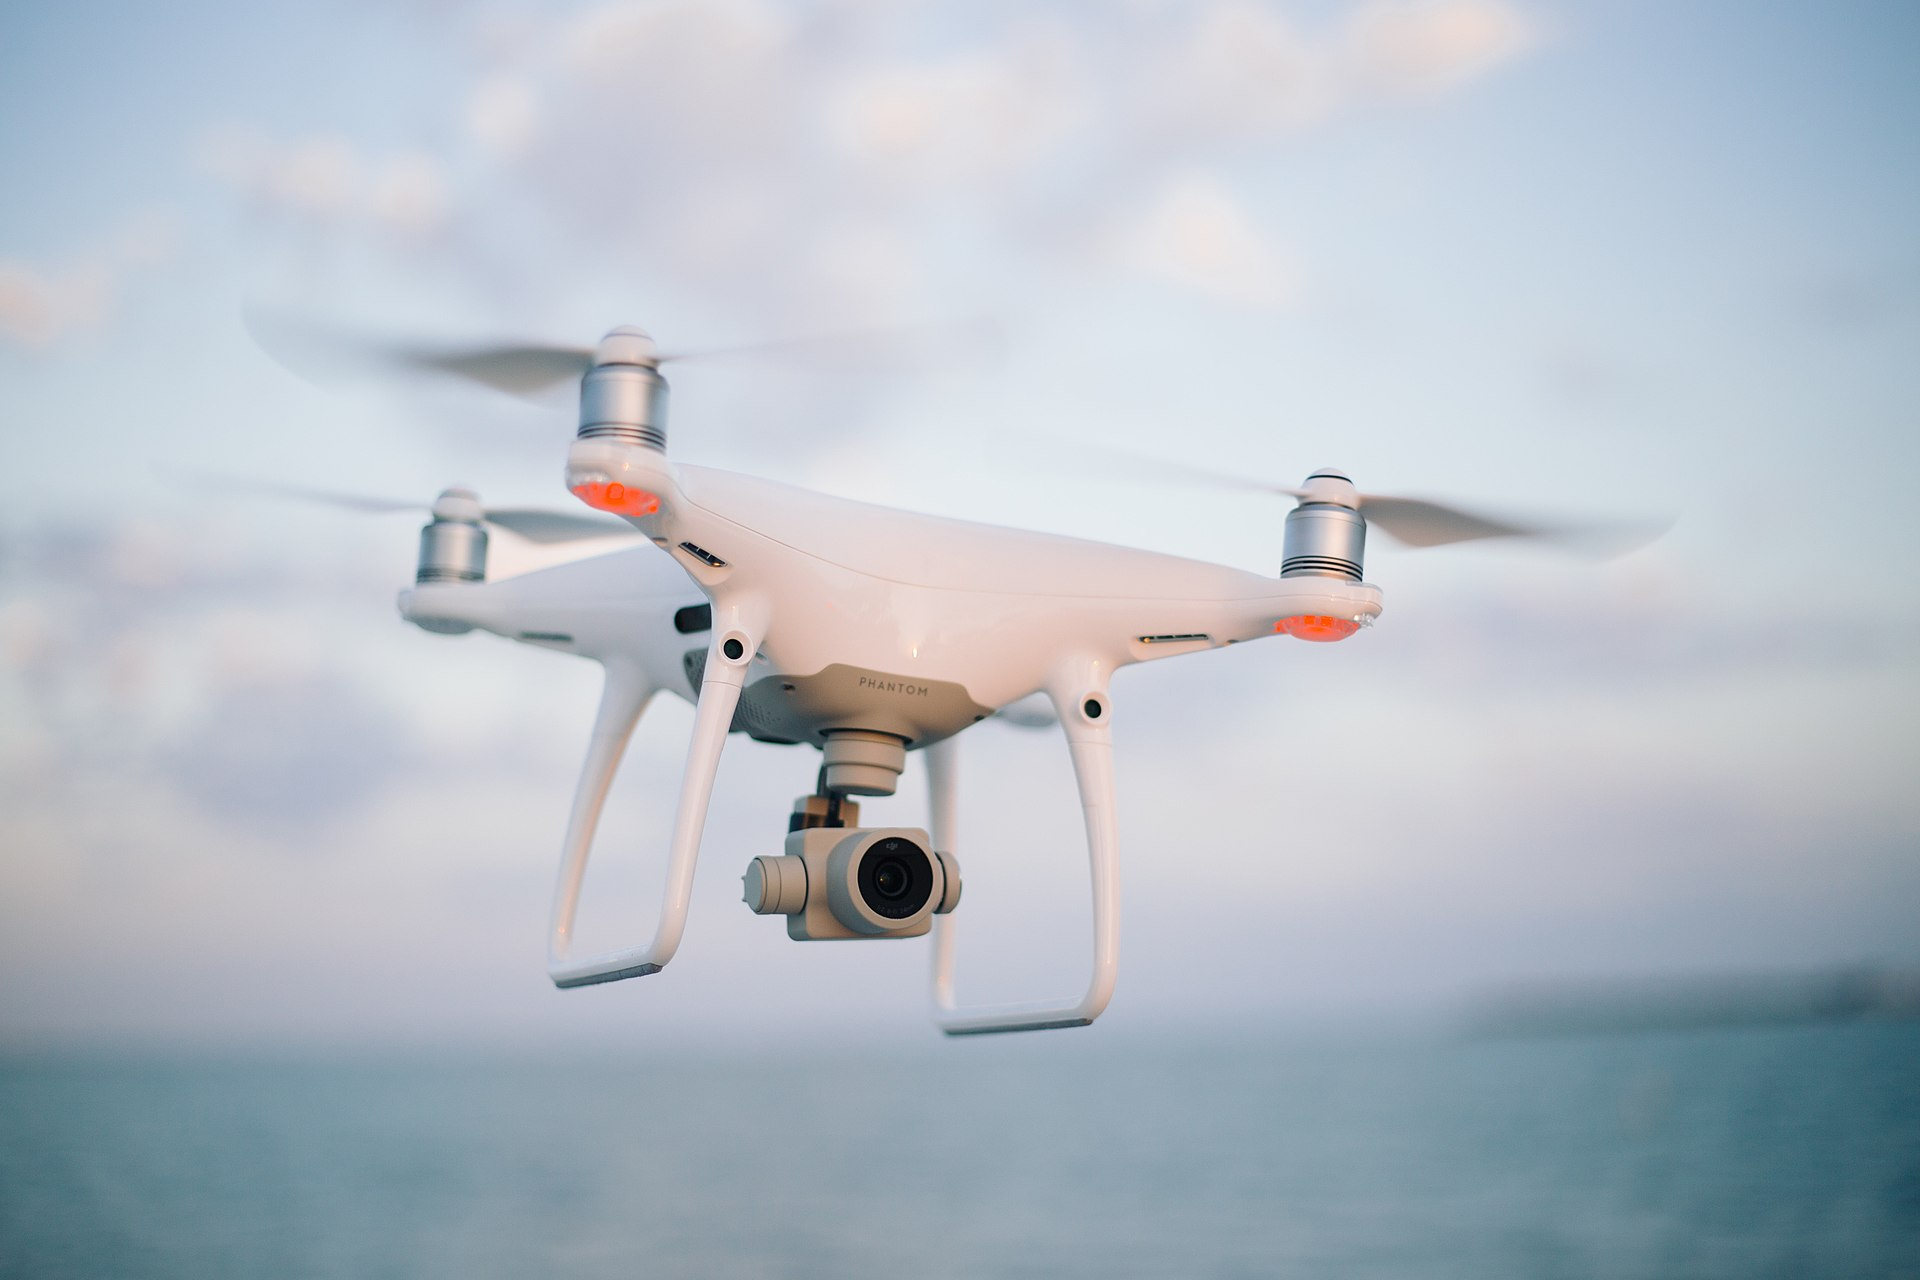
\includegraphics[width=\textwidth]{Images/Introduction/drone}
         \caption[Caption for LOF]{DJI Phantom quadcopter (UAV) \cite{DJIPhantom}.}
         \label{fig:drone}
     \end{subfigure}
     \hfill
     \begin{subfigure}[b]{0.45\textwidth}
         \centering
         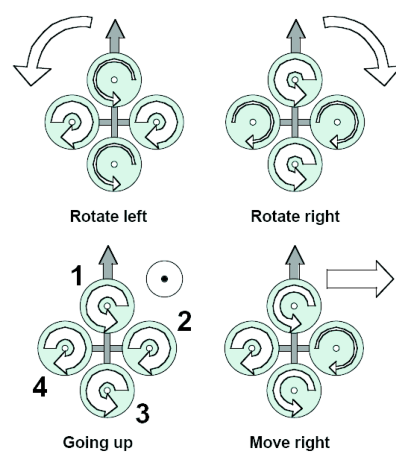
\includegraphics[width=0.6\textwidth]{Images/Introduction/propeller_direction.svg}
         \caption{Quadrotor Concept. Width of the arrows is proportional to the angular speed of the propellers \cite{Bouabdalla2007}.}
         \label{fig:propeller_directions}
     \end{subfigure}
        \caption{Commercial quadrtotor platform (left) and quadrotor concept (right).}
        \label{fig:three graphs}
\end{figure}

\end{frame}

\begin{frame}[t]{Quadrotor Platform} \vspace{4pt}


Properties of the quadrotor:

\begin{itemize}
	\item Under-actuated system.
	\item Controls all DOFs.
\end{itemize}

\vspace{2cm}

	\begin{block}{Remark}
	\vspace{0.5em}
	Rotational and translational dynamics are coupled.
	\vspace{0.5em}
	\end{block}


\end{frame}


\begin{frame}[t]{Goal of The Master Thesis} \vspace{4pt}
Goal of the master thesis: 

\begin{itemize}[<+->]
	\item Study of multi-flip maneuvers.
	\item Use different control methods.
	\item Performing the maneuvers in a constrained environment.
\end{itemize}

\begin{figure}[h]
     \centering
     \begin{subfigure}[h]{0.45\textwidth}
         \centering
         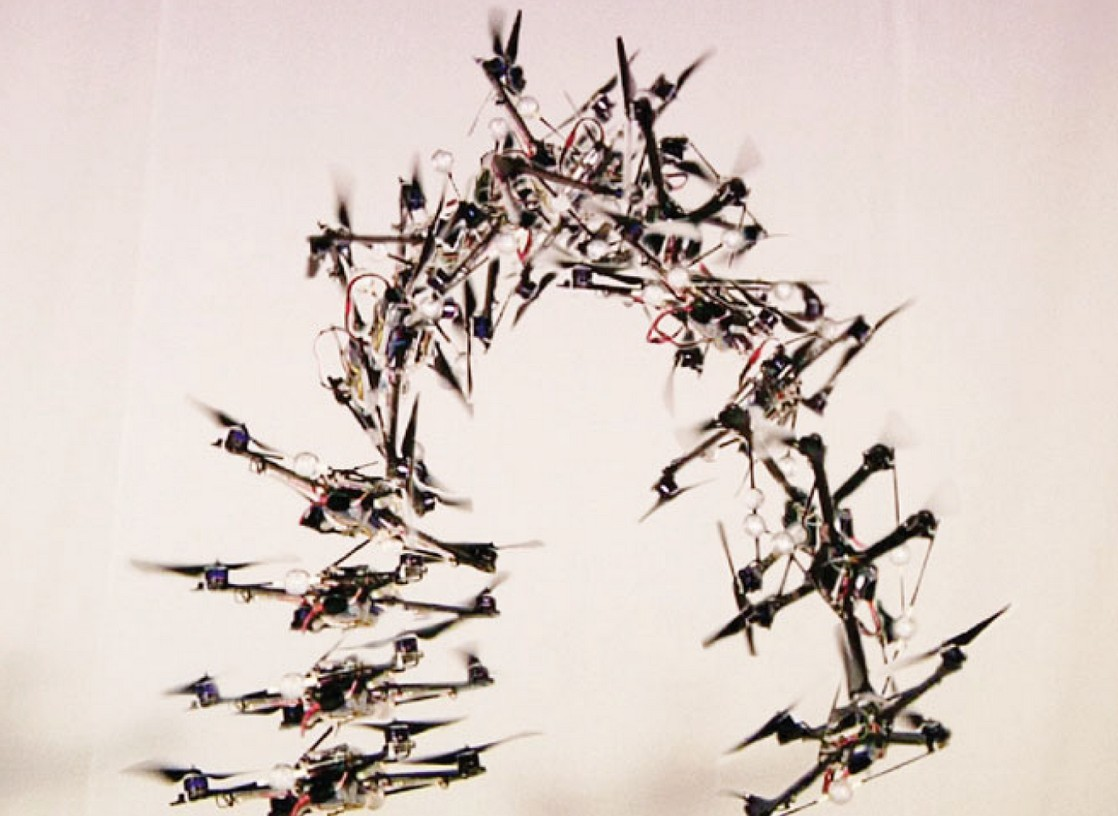
\includegraphics[width=0.9\textwidth]{Images/Introduction/flip}
    \caption{Quadrotor performing a triple flip.\cite{flip}}
         \label{triple_flip}
     \end{subfigure}
     \hfill
     \begin{subfigure}[h]{0.45\textwidth}
         \centering
         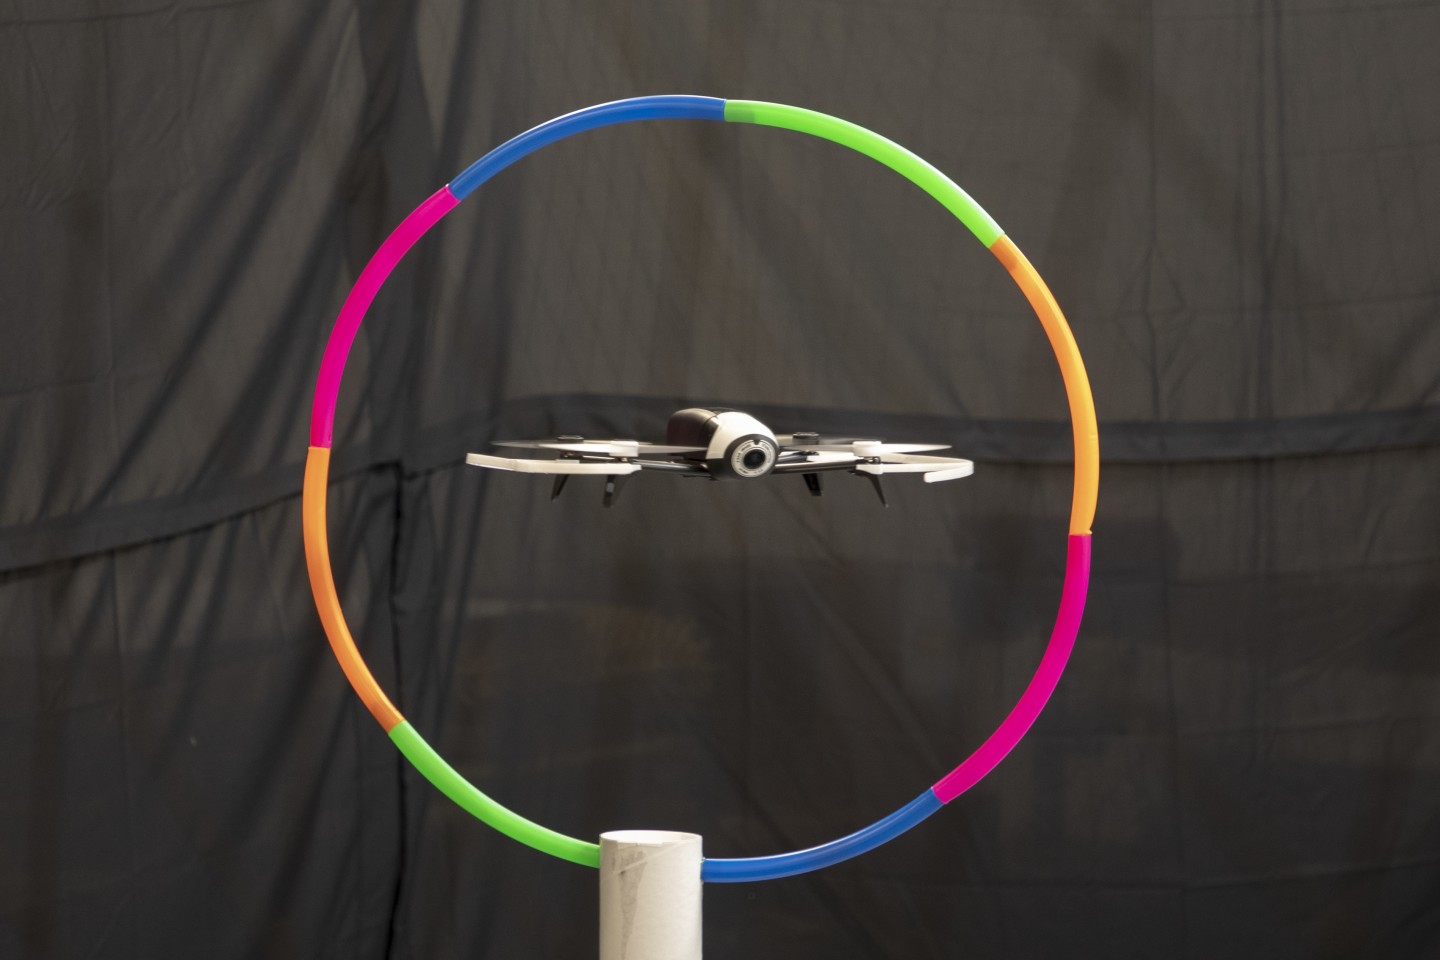
\includegraphics[width=\textwidth]{Images/Introduction/constrained_environment}
         \caption[Caption for LOF]{Quadrotor going though a loop \cite{Coxworth2020}.}
         \label{drone_hulahoop}
     \end{subfigure}
        \caption{Representation of the issues to be tackled in this master thesis.}
        \label{fig:three graphs}
\end{figure}

\end{frame}






\section{System Modeling}

%\subsection{Inputs}
\begin{frame}[t]{Inputs} \vspace{4pt}
Principal \textbf{forces} and \textbf{torques} are generated  by the propellers' rotations.

\begin{itemize}
	\item \textbf{Forces} - Decomposed into 2 parts:
	
	\begin{itemize}
		\item Weight.
		\item Resulting lift.
	\end{itemize}
	
	\begin{equation}
\overrightarrow{F_{\xi}}= \overrightarrow{P} + \sum \overrightarrow{f_i}
\end{equation} 
which results in \cite{Fantoni2016}:

\begin{equation}
\overrightarrow{F_{\xi}} =
\prescript{O}{}{\begin{bmatrix}
0 \\
0 \\
-mg \\
\end{bmatrix}}
+ b \prescript{U}{}{\begin{bmatrix}
0 \\ 
0 \\
\omega_1^2 + \omega_2^2 + \omega_3^2 + \omega_4^2\\
\end{bmatrix}}
\end{equation}
\end{itemize}
\end{frame}

\begin{frame}[t]{Inputs} \vspace{4pt}
\begin{itemize}
	\item \textbf{Torques} - 2 parts:
	\begin{itemize}
		\item Relation between the velocities of the rotors.
		\item Gyroscopic effects due to the change of orientation direction of the rotors.
	\end{itemize}
	
\begin{equation}
	\tau = \tau_a + \tau_G
\end{equation}
which results in \cite{Fantoni2016}:
\begin{equation}\label{total_torque_equation}
\tau = \begin{bmatrix}
\tau_1\\
\tau_2\\
\tau_3\\
\end{bmatrix} = \tau_a + \tau_G = \begin{bmatrix}
l(f_4-f_2) - qJ_r(\omega_1-\omega_2+\omega_3-\omega_4)\\
l(f_3-f_1) + pJ_r(\omega_1-\omega_2+\omega_3-\omega_4)\\
d(\omega_1^2-\omega_2^2+\omega_3^2-\omega_4^2)\\
\end{bmatrix}
\end{equation}
\end{itemize}
\end{frame}


\begin{frame}[t]{Inputs} \vspace{4pt}
Motors are controlled with torques and thrust using 4 control inputs.


\begin{columns}


\column{0.5\textwidth}

\begin{align*}
u_1 &= u \text{ (thrust)}\\
u_2 &= \tau_{\phi} \\
u_3 &= \tau_{\theta} \\
u_4 &= \tau_{\psi}
\end{align*}

\vspace{2cm}

\column{0.5\textwidth}

\begin{figure}[h]
\centering
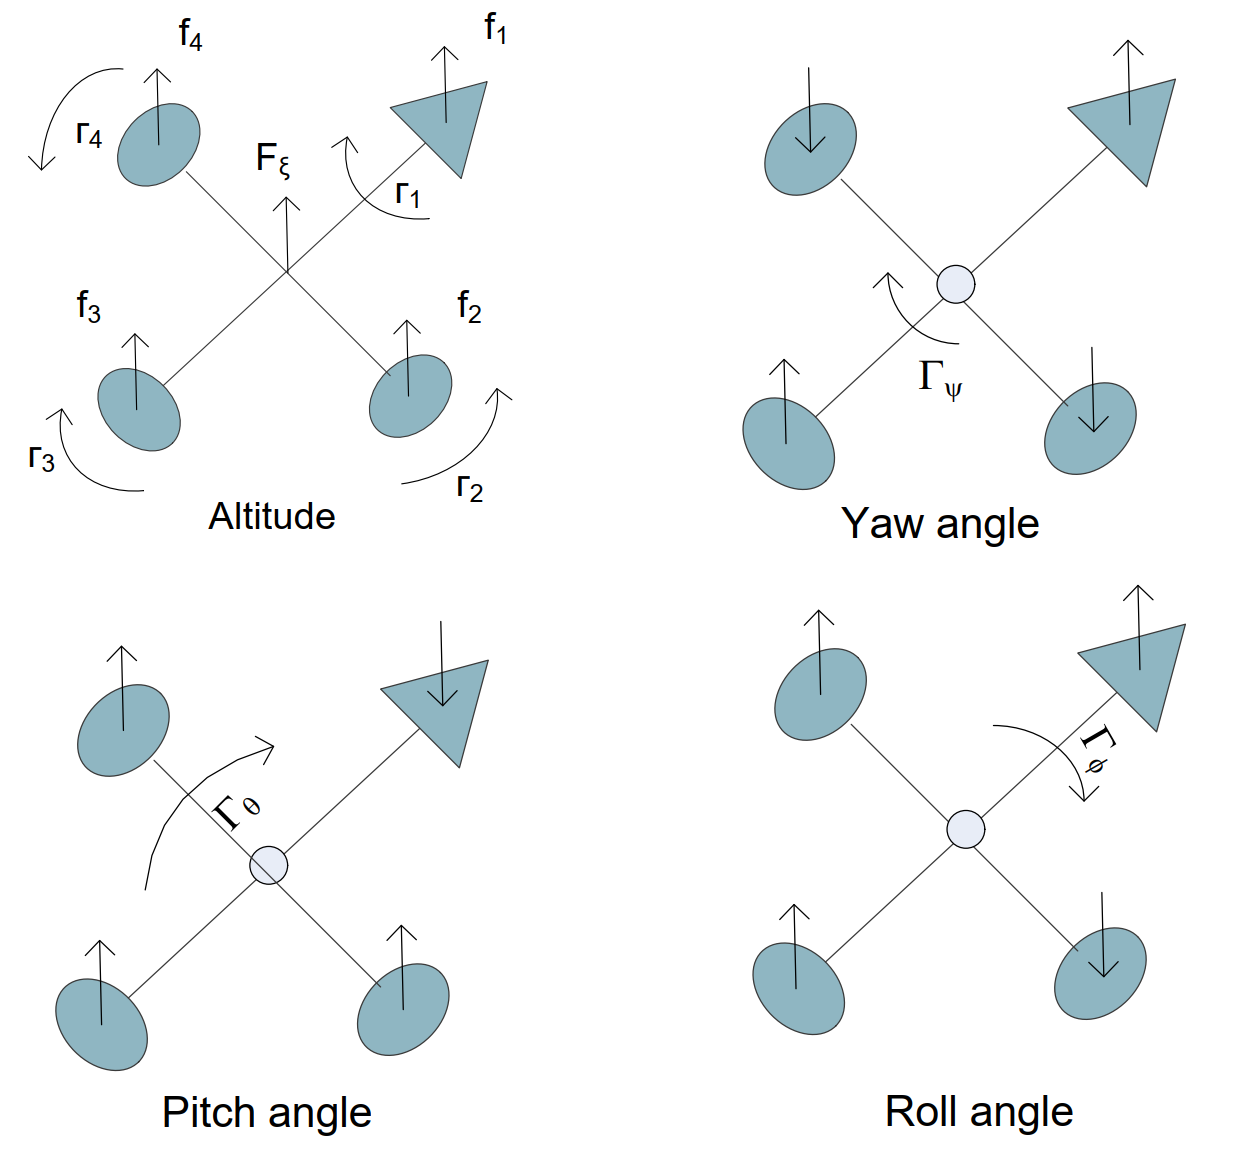
\includegraphics[width=\textwidth]{Images/Modeling/Fantoni_a}
\caption{Quadrotor model with motor torques and Euler angles \cite{Fantoni2016}.}
\label{Fantoni_a}
\end{figure}
\end{columns}
\end{frame}

%\subsection{Dynamic Equations}

\begin{frame}[t]{Dynamic Equations} \vspace{4pt}
First, some assumptions are made:

\begin{itemize}[<+->]
	\item Rigid structure.
	\item Symmetric structure.
	\item CoG and origin of body-fixed frame coincide.
	\item Propellers are rigid.
	\item Thrust and drag are proportional to the square of the velocity of the propeller.
\end{itemize}
\end{frame}


\begin{frame}[t]{Dynamic Equations} \vspace{4pt}

The dynamic model:
\begin{itemize}[<+->]
	\item Computed using \textbf{Euler-Lagrange} or \textbf{Newton-Euler} formalism.
	\item Decomposed to \textbf{2 different parts} \cite{Fantoni2016}:
		\begin{itemize}
			\item \textbf{Translational} model:

\begin{equation}\label{translation_model_N_E}
\begin{cases}
m \ddot{x} = (\sin \psi \sin \phi + \cos \psi \sin \theta \cos \phi)u \\
m \ddot{y} = (- \sin \phi \cos \psi + \sin \psi \sin \theta \cos \phi )u \\
m \ddot{z} = \cos \theta \cos \phi u -mg \\
\end{cases}
\end{equation}			
			
			\item \textbf{Rotational} model:

\begin{equation}
\begin{cases}
\dot{p} = qr \frac{(I_{yy}-I_{zz})}{I_{xx}} + \frac{l}{I_{xx}}(f_4-f_2) - \frac{1}{I_{xx}}qJ_r (\omega_1 - \omega_2 + \omega_3 - \omega_4) \\
\dot{q} = pr \frac{(I_{zz}-I_{xx})}{I_{yy}} + \frac{l}{I_{yy}}(f_3-f_1) + \frac{1}{I_{yy}}pJ_r (\omega_1 - \omega_2 + \omega_3 - \omega_4) \\
\dot{r} = pq \frac{(I_{xx}-I_{yy})}{I_{zz}} + \frac{1}{I_{zz}} d (\omega_1^2 -\omega_2^2 + \omega_3^2 - \omega_4^2)
\end{cases}
\end{equation}			
		\end{itemize}
\end{itemize}
\end{frame}


\begin{frame}[t]{Dynamic Equations} \vspace{4pt}
For small pitch and roll angles of order 2, a simplified dynamic model is obtained: 

\begin{itemize}
	\item \textbf{Translational} model:
\begin{equation}\label{translational_model_E_L_Simplified}
\begin{cases}
m \ddot{x} = (\phi \sin \psi + \theta \cos \psi)u \\
m \ddot{y} = (- \phi \cos \psi + \theta \sin \psi)u \\
m \ddot{z} = u - mg \\
\end{cases}
\end{equation}
	\item \textbf{Rotational} model:
\begin{equation}\label{N_E_rotation_equation_small_angles}
\begin{cases}
\ddot{\phi} = \dot{\theta} \dot{\psi} \frac{(I_{yy}-I_{zz})}{I_{xx}} + \frac{l}{I_{xx}}(f_4-f_2) - \frac{1}{I_{xx}} \dot{\theta} J_r (\omega_1 - \omega_2 + \omega_3 - \omega_4) \\
\ddot{\theta} = \dot{\psi} \dot{\phi} \frac{(I_{zz}-I_{xx})}{I_{yy}} + \frac{l}{I_{yy}}(f_3-f_1) + \frac{1}{I_{yy}} \dot{\phi} J_r (\omega_1 - \omega_2 + \omega_3 - \omega_4) \\
\ddot{\psi} = \dot{\theta} \dot{\phi} \frac{(I_{xx}-I_{yy})}{I_{zz}} + \frac{1}{I_{zz}} d (\omega_1^2 -\omega_2^2 + \omega_3^2 - \omega_4^2)
\end{cases}
\end{equation}	
\end{itemize}

\end{frame}

\begin{comment}
\begin{frame}[t]{State-Space Representation} \vspace{4pt}
The system can be written in state-space form $\dot{\textbf{\textsc{x}}}=f(\textbf{\textsc{x}},\textbf{\textsc{u}})$

\begin{equation}\label{state_vector}
\textbf{\textsc{x}} = \left[\begin{array}{c c c c c c c c c c c c c}
\phi & \dot{\phi} & \theta & \dot{\theta} & \psi & \dot{\psi} & z & \dot{z} & x & \dot{x} & y & \dot{y} 
\end{array}\right]^{\intercal}
\end{equation}
with
\begin{multicols}{2}
 
\begin{equation*}
\begin{aligned}
x_1 = \phi\\
x_2 = \dot{x}_1=\dot{\phi}\\
x_3 = \theta\\
x_4 = \dot{x}_3 = \dot{\theta} \\
x_5 = \psi \\
x_6 = \dot{x}_5 = \dot{\psi}\\
\end{aligned}
\end{equation*}

\columnbreak

\begin{equation}
\begin{aligned}
x_7 = z\\
x_8 = \dot{x}_7=\dot{z}\\
x_9 = x\\
x_{10} = \dot{x}_9 = \dot{x} \\
x_{11} = y \\
x_{12} = \dot{x}_{11} = \dot{y}\\
\end{aligned}
\end{equation}

\end{multicols}

\end{frame}

\begin{frame}[t]{State-Space Representation} \vspace{4pt}
And,
\begin{equation}\label{control_input_vector}
\textbf{\textsc{u}} = \left[\begin{array}{c c c c}
u_1 & u_2 & u_3 & u_4 
\end{array}\right]^{\intercal}
\end{equation}

Where the control inputs are mapped by: 

\begin{equation}\label{Control_input_mapping}
\begin{cases}
u_1 = b(\omega_1^2 + \omega_2^2 + \omega_3^2 + \omega_4^2)\\
\\
u_2 = b(-\omega_2^2 + \omega_4^2)\\
\\
u_3 = b(\omega_1^2 - \omega^3)\\
\\
u_4 = d(-\omega_1^2 + \omega_2^2 - \omega_3^2 + \omega_4^2) \\
\end{cases}
\end{equation}
\end{frame}

\begin{frame}[t]{State-Space Representation} \vspace{4pt}
For small angles, $(\dot{\phi},\dot{\theta},\dot{\psi})  \approx (p,q,r)$, the system becomes:

\begin{equation}\label{state_space_model}
f(\textbf{\textsc{x}},\textbf{\textsc{u}}) = \begin{pmatrix}
\dot{\phi}\\
\dot{\theta} \dot{\psi} a_1 + \dot{\theta} a_2 \Omega_r + b_1 u_2 \\
\dot{\theta}\\
\dot{\phi} \dot{\psi} a_3 - \dot{\phi} a_4 \Omega_r + b_2 u_3 \\
\dot{\psi}\\
\dot{\theta} \dot{\psi} a_5 + b_3 u_4 \\
\dot{z}\\
g - (\cos \phi \cos \theta) \frac{1}{m} u_1 \\
\dot{x} \\
u_x \frac{1}{m} u_1\\
\dot{y}\\
u_y \frac{1}{m}u_1\\
\end{pmatrix}
\end{equation}

\end{frame}


\begin{frame}[t]{State-Space Representation} \vspace{4pt}

With, 

\begin{multicols}{2}
 
\begin{equation*}
\begin{aligned}
a_1 &= (I_{yy} - I_{zz})/I_{xx}\\
a_2 &= J_r/I_{xx}\\
a_3 &= (I_{zz} - I_{xx})/I_{yy}\\
a_4 &= J_r/I_{yy}\\
a_5 &= (I_{xx} - I_{yy})/I_{zz}\\
\end{aligned}
\end{equation*}

\columnbreak

\begin{equation}
\begin{aligned}
b_1 &= l/I_{xx}\\
b_2 &=l/I_{yy}\\
b_3 &= l/I_{zz}\\
\end{aligned}
\end{equation}

\end{multicols}

\begin{equation}
	\begin{aligned}
	u_x = (\cos \phi \sin \theta \cos \psi + \sin \phi \sin \psi)\\
	u_y = (\cos \phi \sin \theta \sin \psi - \sin \phi \cos \psi)\\
	\end{aligned}
\end{equation}

\end{frame}


\begin{frame}[t]{State-Space Representation} \vspace{4pt}

In this system, the angles and their derivatives do not depend on the translation components.

\begin{figure}[h]
\centering 
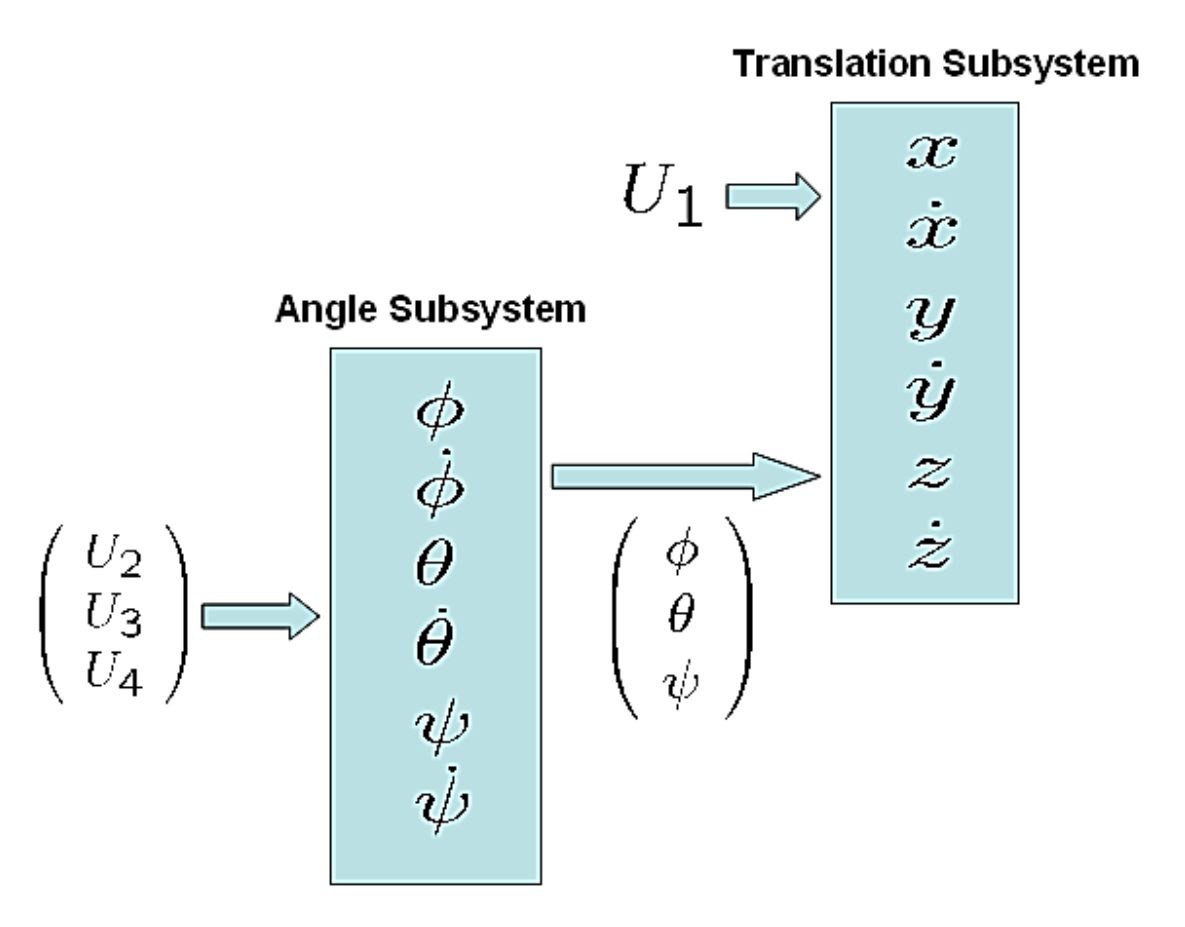
\includegraphics[width=0.5\textwidth]{Images/Modeling/subsystems}
\caption{Link between the rotation and the translation subsystems \cite{Bouabdalla2007}.}
\end{figure}

\end{frame}
\end{comment}

%\subsection{State-Space}


\section{Control of Quadrotors}

\begin{frame}[t]{General Control Architecture} \vspace{4pt}
 \begin{figure}[h]
 \centering
 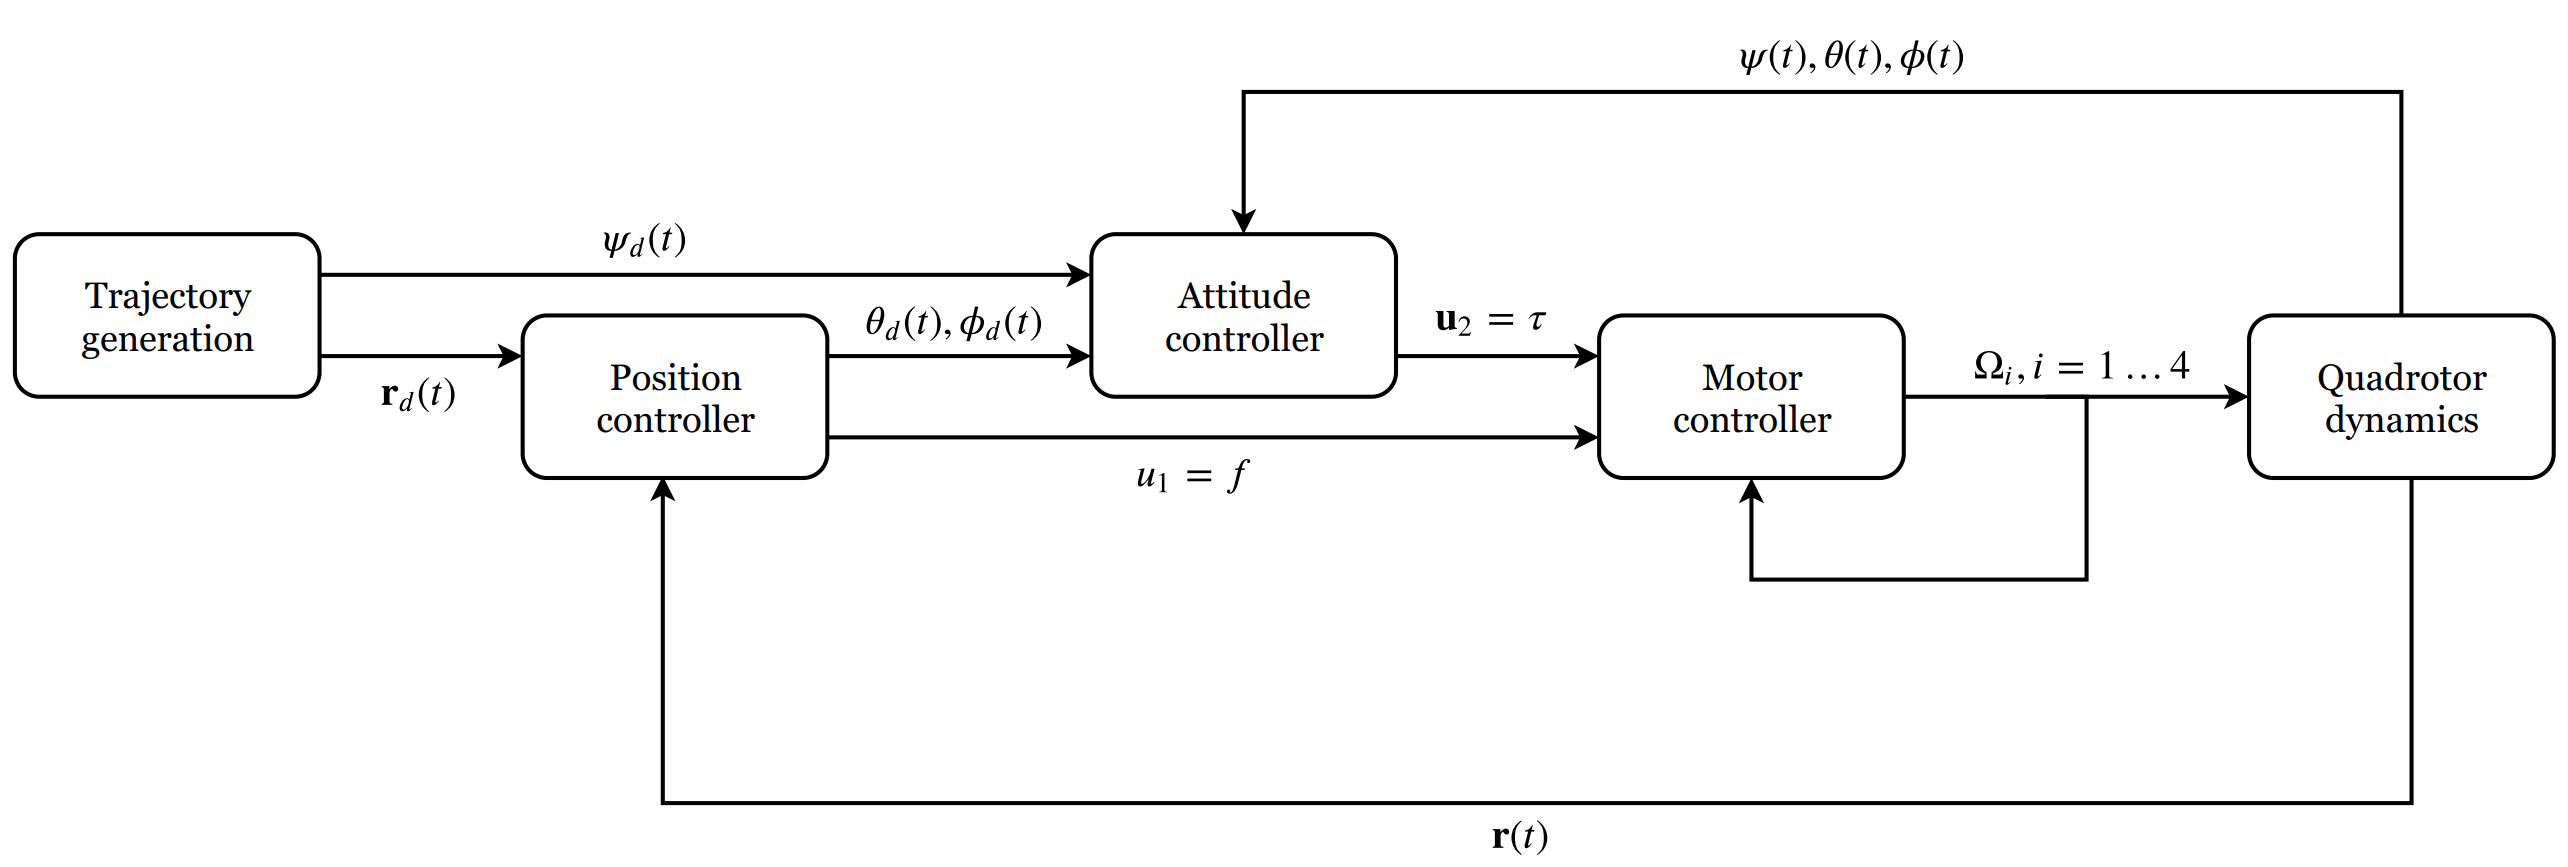
\includegraphics[width=0.8\textwidth]{Images/Control/General_control_architecture}
 \caption{General control architecture for the position and attitude of a quadrotor \cite{Faessler2018}.}
 \end{figure}
 
\begin{itemize}[<+->]
	\item \textbf{Position controller}: drives translational dynamics errors to 0.
	\item \textbf{Attitude controller}: drives rotational dynamics errors to 0.
	\item \textbf{Motor controller}: receives the control intputs $\bm{u}=\begin{bmatrix}
	f && \bm{\tau}
	\end{bmatrix}^{\intercal}
	$ and maps them to $\Omega_i^*$ for each rotor. %based on \ref{Control_input_mapping}.
\end{itemize} 
\end{frame}

\begin{frame}[t]{Model Predictive Control} 
What is MPC?

 \begin{figure}[t]
 \centering
 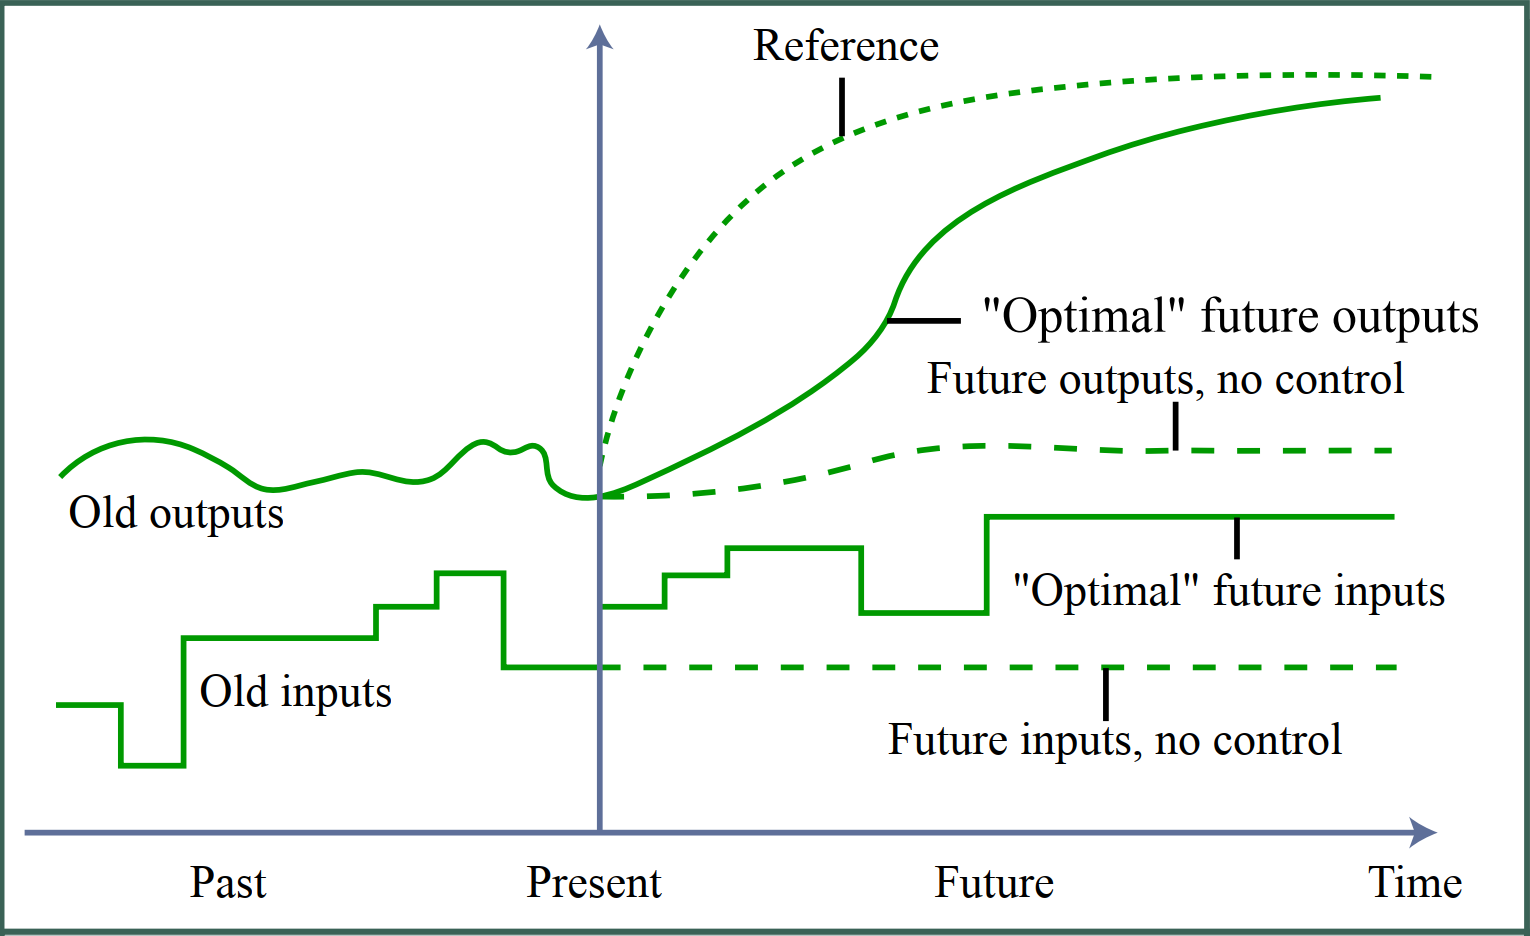
\includegraphics[width=0.5\textwidth]{Images/control/MPC_general_idea}
 \caption{Basic idea of MPC \cite{How2008}.}
 \label{MPC_basic_idea}
\end{figure}  



\begin{itemize}[<+->]
	\item It is a \textbf{feedback control} algorithm.
	\item It uses a model to \textbf{precit} future outputs.
	\item It \textbf{Solves an online optimization problem} to select the optimal control.
\end{itemize}
\end{frame}

\begin{frame}[t]{Model Predictive Control}
\begin{columns}

\column{0.5\textwidth}

\begin{figure}[t]
	\centering
	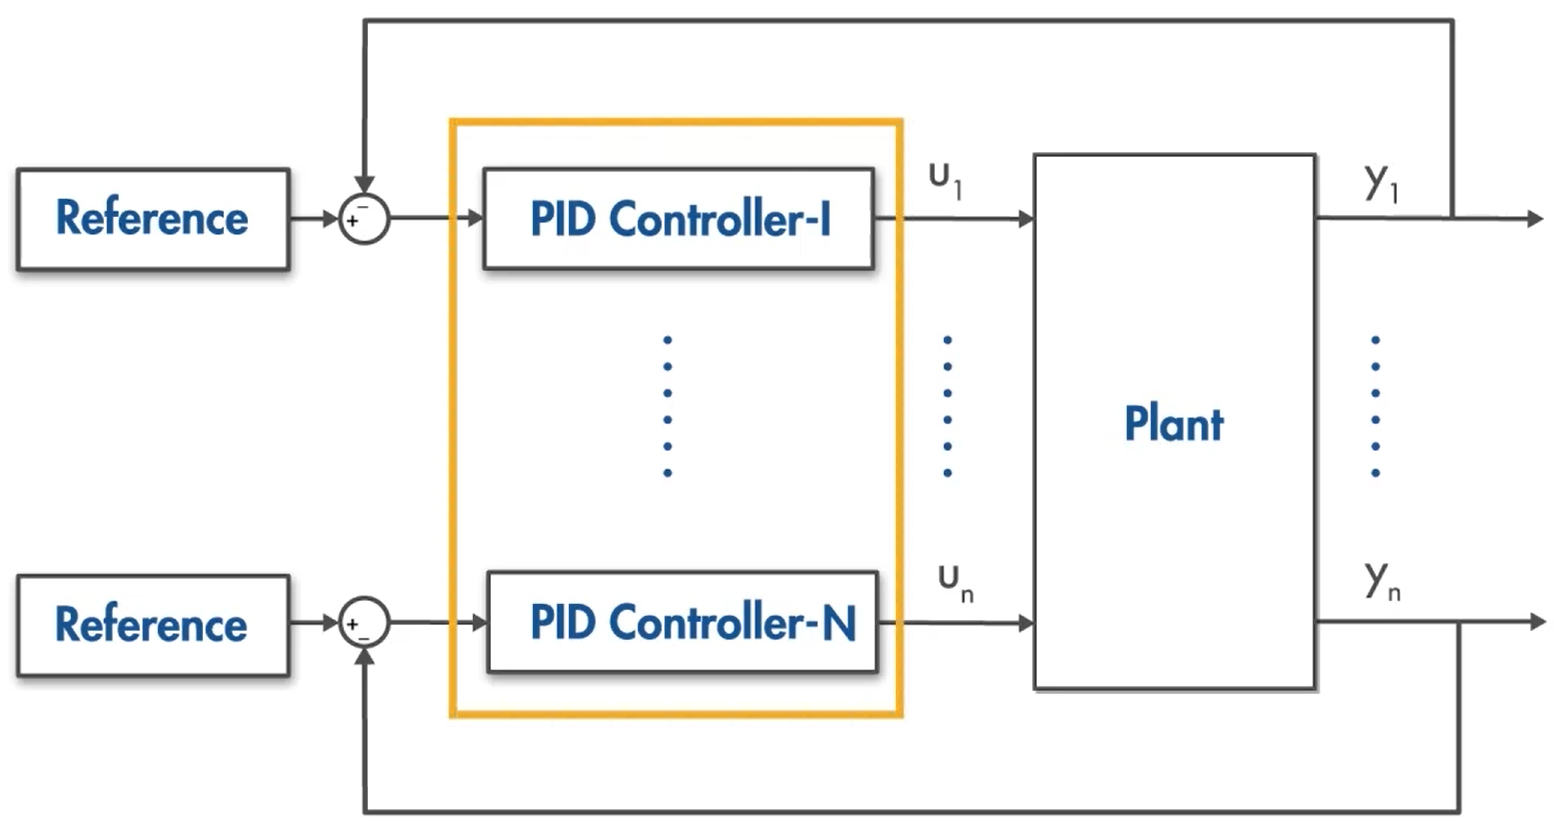
\includegraphics[width=\textwidth]{Images/Control/5}
	\caption{MIMO system with PIDs \cite{MathWorks2018_new}.}
\end{figure}

\column{0.5\textwidth}

\begin{figure}[t]
	\centering
	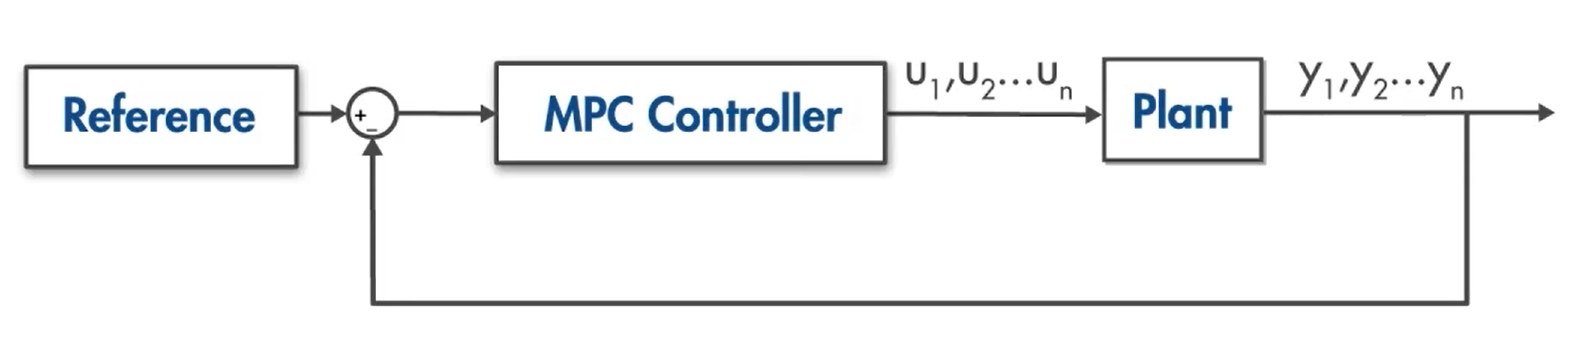
\includegraphics[width=\textwidth]{Images/Control/6}
	\caption{MIMO system with MPC controller \cite{MathWorks2018_new}.}
\end{figure}

\end{columns}





\begin{columns}
\column{0.5\textwidth}
\begin{itemize}[<+->]
	\item Can \textbf{control MIMO} systems.
	\item Explicitly \textbf{accounts for constraints}.
	\item Can handle \textbf{nonlinear and time-varying plant dynamics}.

\vspace{3cm}	
	
\end{itemize}

\column{0.5\textwidth}
\begin{alertblock}{Remark}
\vspace{0.5em}
MPC requires a \textbf{powerful}, \textbf{fast} processor with a \textbf{large} memory.
\vspace{0.5em}
\end{alertblock}

\vspace{3cm}

\end{columns}
\end{frame}

\begin{frame}{Model Predictive Control} \vspace{4pt}

\begin{columns}
\column {0.5\textwidth}
MPC Design parameters:

\begin{itemize}[<+->]
	\item Sample time
	\item Prediction horizon
	\item Control horizon
	\item Constraints
	\item Weights
\end{itemize}\pause


\column {0.5\textwidth}
Choosing proper values for these parameters is important as they affect: 
\begin{itemize}
	\item The controller performance.
	\item The computational complexity of the MPC algorithm.
\end{itemize} 
\end{columns}

\end{frame}

\begin{frame}[t]{Model Predictive Control} \vspace{4pt}
General MPC methods:

\begin{itemize}[<+->]
	\item Linear time-invariant MPC.
	\item Adaptive MPC.
	\item Gain-Scheduled MPC.
	\item Nonlinear MPC.
\end{itemize}

\end{frame}


\begin{frame}{Model Predictive Control} \vspace{4pt}
\textbf{In Adaptive MPC:}
\begin{itemize}
	\item A linear model is computed on the fly as the operating conditions change.
	\item At each time step, the internal plant model used by the MPC is updated with this linear model.
\end{itemize}

\begin{figure}
	\centering	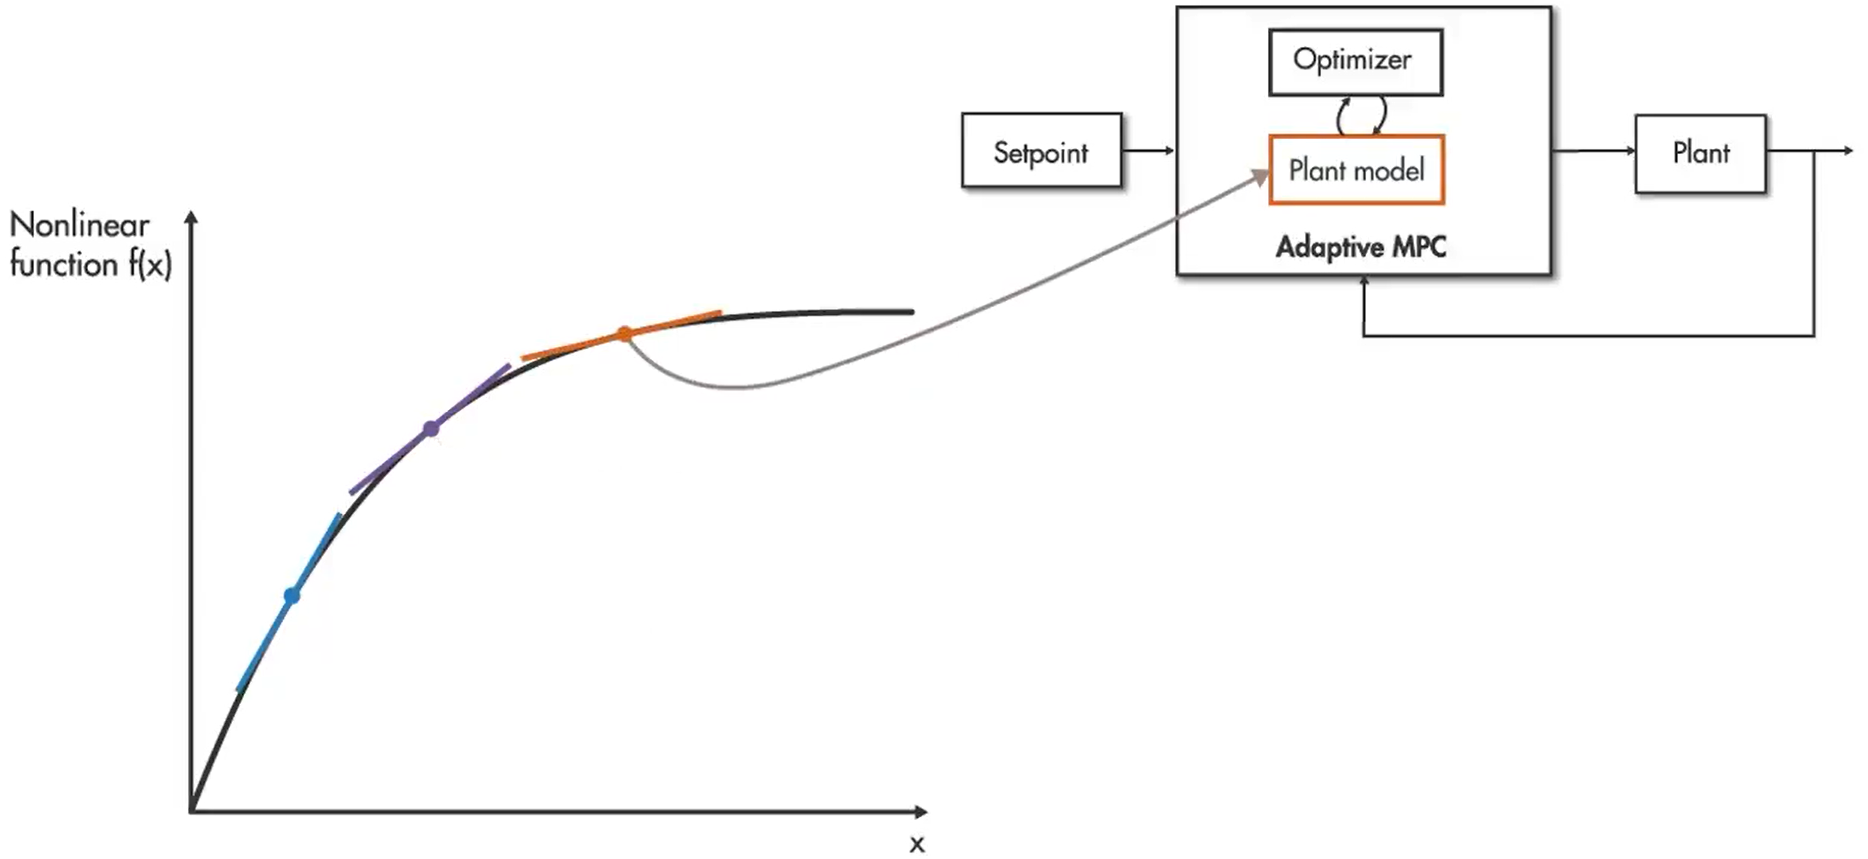
\includegraphics[width=0.7\textwidth]{Images/Control/MPC_adaptive_a}
	\caption{Example of Adaptive MPC \cite{MathWorks_adaptive}.}
\end{figure}

\end{frame}

\begin{frame}{Model Predictive Control} \vspace{4pt}
\begin{alertblock}{Remark}
\vspace{0.5em}
The structure of the optimization problem remains the same across different operating points.
\vspace{0.5em}
\end{alertblock}

\begin{figure}
	\centering	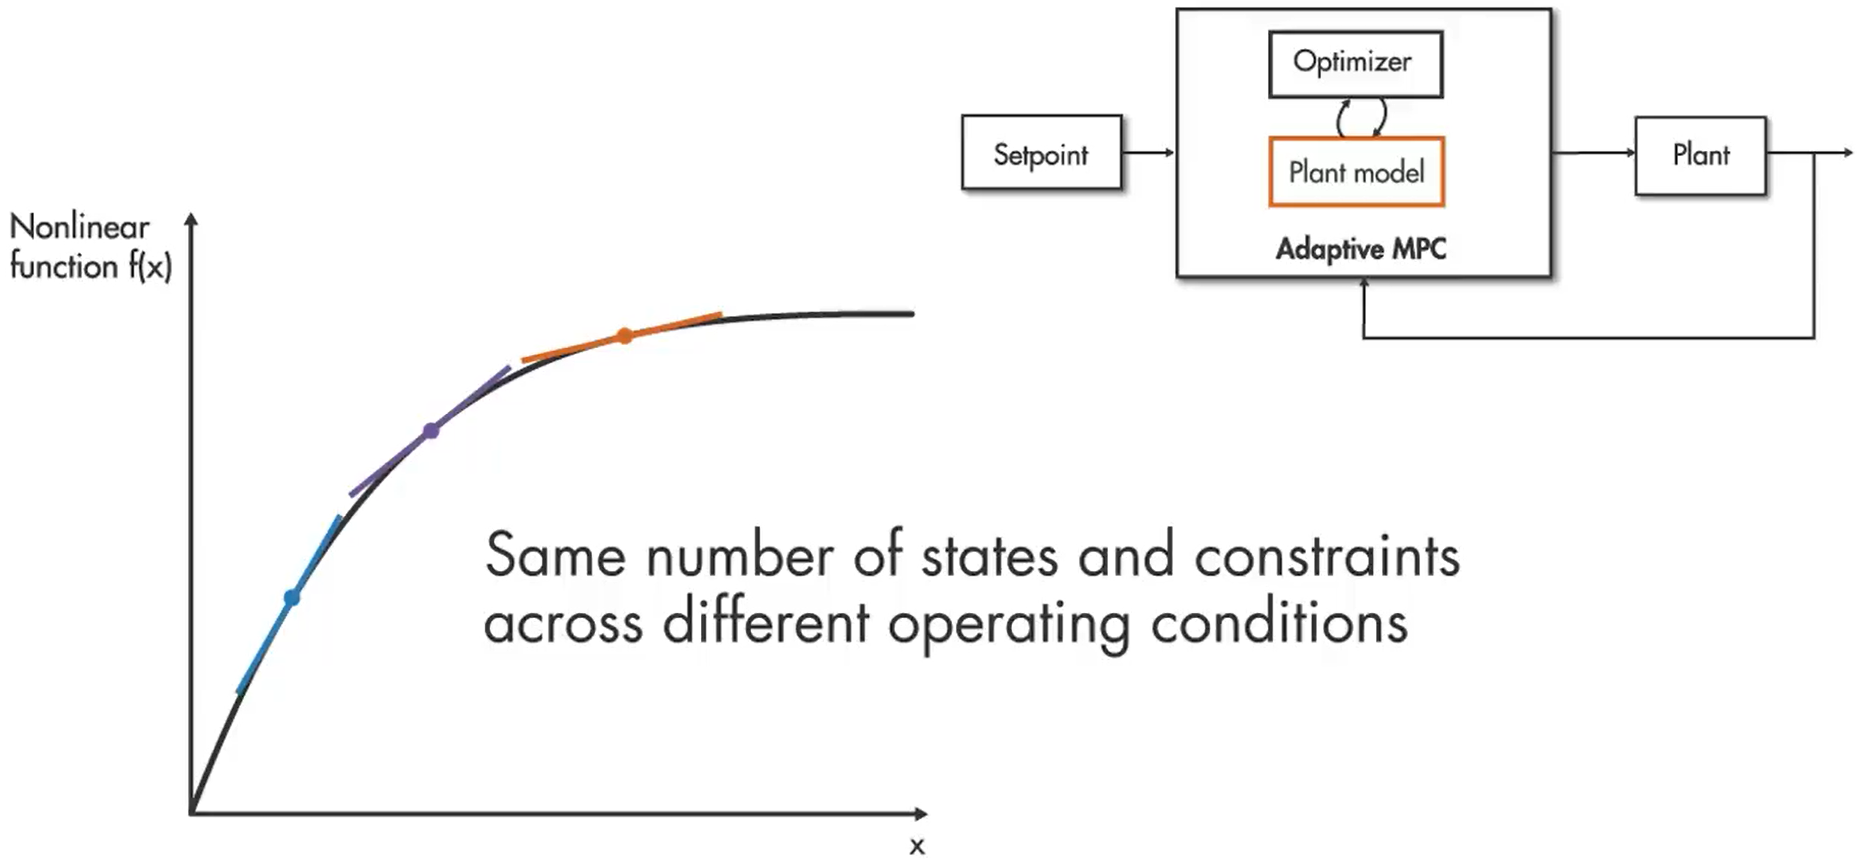
\includegraphics[width=0.7\textwidth]{Images/Control/MPC_adaptive_b}
	\caption{Example of Adaptive MPC \cite{MathWorks_adaptive}.}
\end{figure}

\end{frame}

\begin{frame}{Model Predictive Control} \vspace{4pt}
\textbf{In Gain-Scheduled MPC:}
\begin{itemize}
	\item Linearization is done offline at the operating points of interest.
	\item A linear MPC controller is then designed for each operating point.
\end{itemize}

\begin{figure}
	\centering	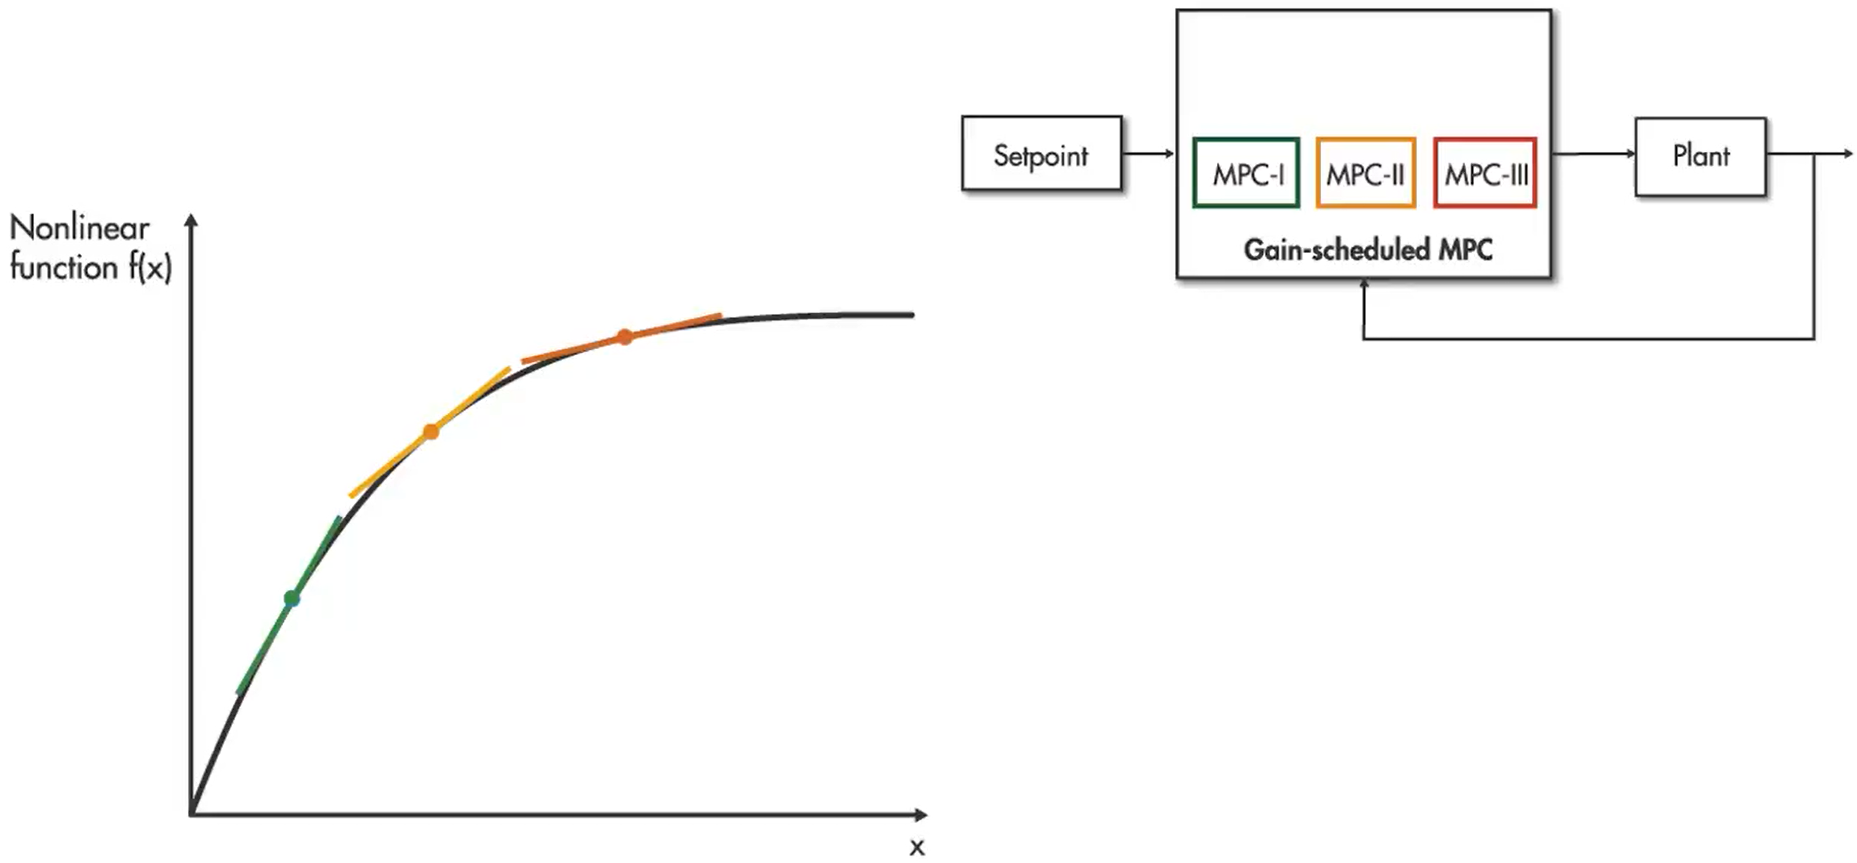
\includegraphics[width=0.7\textwidth]{Images/Control/MPC_gain_a}
	\caption{Example of Gain-Scheduled MPC \cite{MathWorks_adaptive}.}
\end{figure}
\end{frame}

\begin{frame}{Model Predictive Control} \vspace{4pt}
\begin{alertblock}{Remark}
\vspace{0.5em}
Each controller is \textbf{independent} from the other.
\vspace{0.5em}
\end{alertblock}

\begin{figure}
	\centering	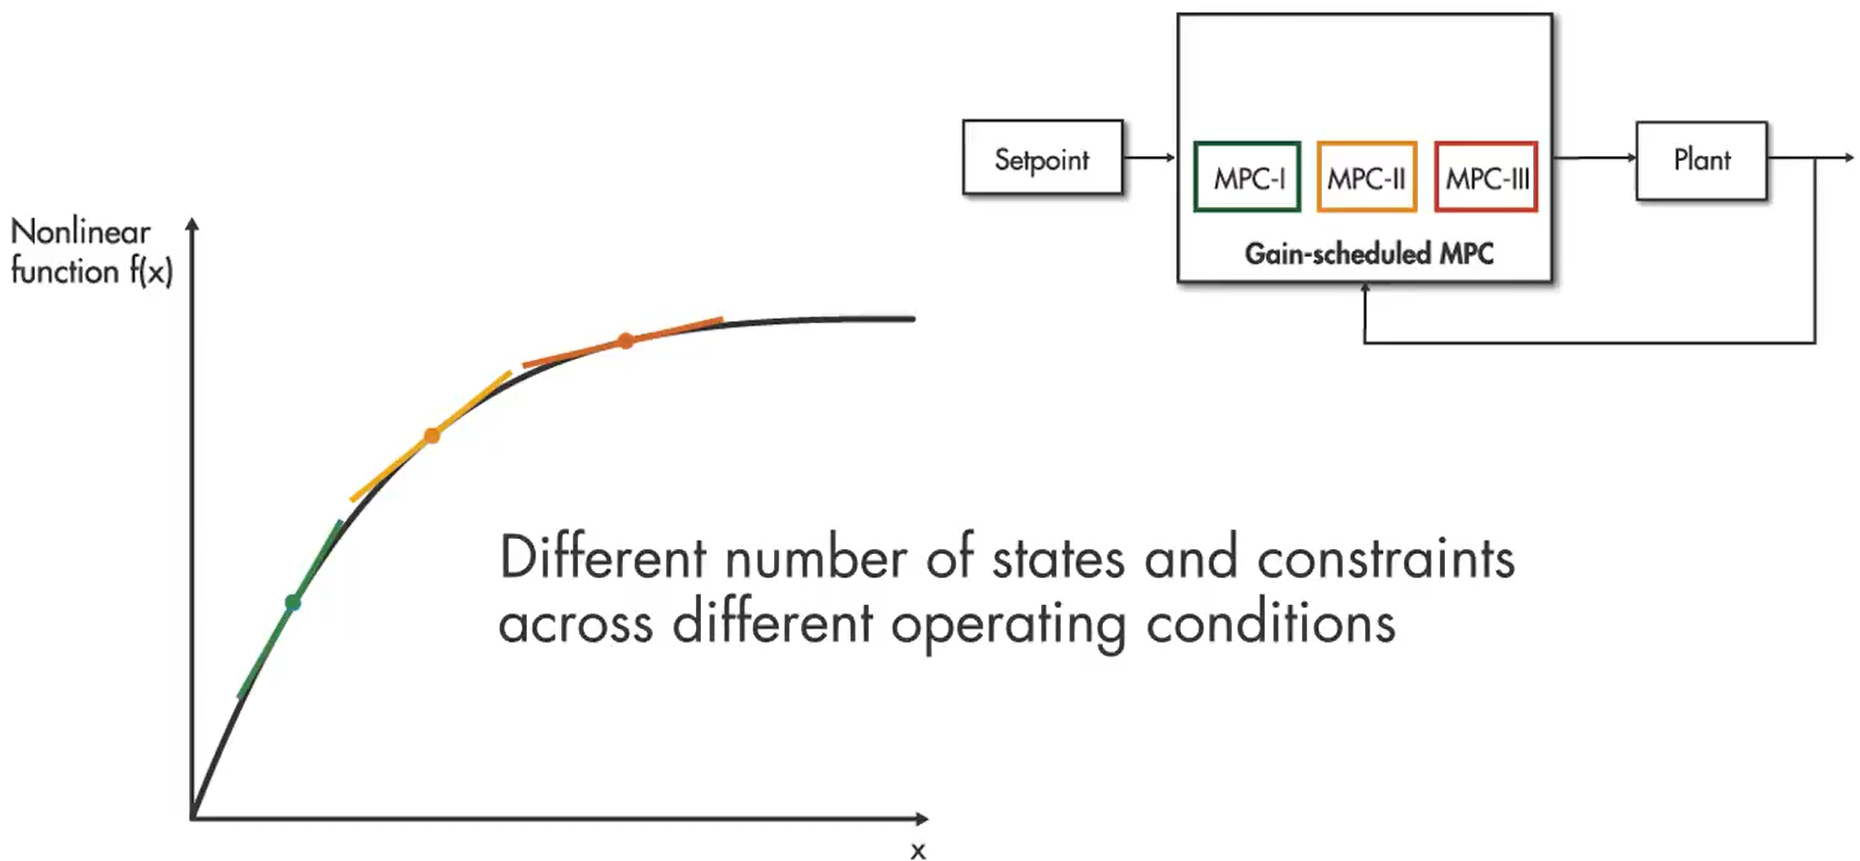
\includegraphics[width=0.7\textwidth]{Images/Control/MPC_gain_b}
	\caption{Example of Gain-Scheduled MPC \cite{MathWorks_adaptive}.}
\end{figure}

\end{frame}

\begin{frame}[t]{Model Predictive Control} \vspace{4pt}

\begin{columns}

\column{0.5\textwidth}

For \textbf{Nonlinear MPC}, useful if:
\begin{itemize}
	\item System is \textbf{non-linearizable}.
	\item Existence of \textbf{nonlinear} constraints.
	\item Existence of \textbf{nonlinear} cost function.
\end{itemize}

\column{0.5\textwidth}

\begin{block}{Nonlinear MPC}

\vspace{0.5em}
Most powerful methods: uses the most accurate representation of the plant $\Rightarrow$ \textbf{More accurate predictions}.
\vspace{0.5em}

\end{block}
\end{columns}


\begin{figure}
	\centering	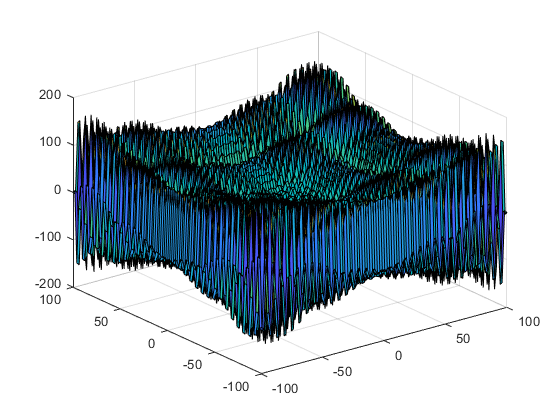
\includegraphics[width=0.4\textwidth]{Images/Control/MPC_Nonconvex_Equation_b}
	\caption{Example of a non-convex optimization problem.}
\end{figure}


\end{frame}



%\subsection{Differntial Flatness}
%\subsection{General Control Architecture}
%\subsection{Model Predictive Control}
%\subsection{Other Control Methods}

\section{Multi-Flip Maneuvers with Quadrotors}
%\subsection{Physics of a quadrotor flip}
%\subsection{Shortcoming of Current Strategies}

\section{Trajectory Optimization}
%\subsection{Introduction}
%\subsection{Trapezoidal collocation}
%\subsection{Hermite-Simpson collocation}










\begin{comment}
\begin{frame}{Equations}
\begin{itemize}[<+->]
  \item Have a number if used with \texttt{\textbackslash{begin}\{equation\}} \cite{Bouabdalla2007}
  \begin{equation}
  \forall \phi: \quad \cos ^2 \phi + \sin^2\phi = 1
  \end{equation}\vfill
  \item Do not have a numbers if used with \texttt{\textbackslash{begin}\{equation*\}}
    \begin{equation*}
  \forall a, b: \quad (a+b)^2 = a^2 + 2ab + b^2
  \end{equation*}
    \item Another useful environment is simply  \texttt{\textbackslash{begin}\{center\}}
    \begin{center}
    $\forall a, b: \quad (a-b)^2 = a^2 - 2ab + b^2$
    \end{center}
    \begin{itemize}[<+->]
    \item Probably more suited to slides as we use less equation references
  \end{itemize} \vfill\vfill   
  \item Can also be included in the text / bullets
  \begin{itemize}[<+->]
    \item $\forall \phi: \quad  (\cos\phi+\sin\phi)^2 = 2\cos\phi\sin\phi + 1$
  \end{itemize}
\end{itemize}
\end{frame}
\end{comment}


\section{References}

\begin{frame}[t,allowframebreaks]{References} \vspace{4pt}

\printbibliography

\end{frame}

\end{document}
